\documentclass[12pt]{article}
 
\usepackage[margin=1in]{geometry}
\usepackage{amsmath,amsthm,amssymb}
\usepackage{mathtools}
\DeclarePairedDelimiter{\ceil}{\lceil}{\rceil}
%\usepackage{mathptmx}
\usepackage{accents}
\usepackage{comment}
\usepackage{graphicx}
\usepackage{IEEEtrantools}
 \usepackage{float}
 
\newcommand{\N}{\mathbb{N}}
\newcommand{\Z}{\mathbb{Z}}
\newcommand{\R}{\mathbb{R}}
\newcommand{\Q}{\mathbb{Q}}
\newcommand*\conj[1]{\bar{#1}}
\newcommand*\mean[1]{\bar{#1}}
\newcommand\widebar[1]{\mathop{\overline{#1}}}


\newcommand{\cc}{{\mathbb C}}
\newcommand{\rr}{{\mathbb R}}
\newcommand{\qq}{{\mathbb Q}}
\newcommand{\nn}{\mathbb N}
\newcommand{\zz}{\mathbb Z}
\newcommand{\aaa}{{\mathcal A}}
\newcommand{\bbb}{{\mathcal B}}
\newcommand{\rrr}{{\mathcal R}}
\newcommand{\fff}{{\mathcal F}}
\newcommand{\ppp}{{\mathcal P}}
\newcommand{\eps}{\varepsilon}
\newcommand{\vv}{{\mathbf v}}
\newcommand{\ww}{{\mathbf w}}
\newcommand{\xx}{{\mathbf x}}
\newcommand{\ds}{\displaystyle}
\newcommand{\Om}{\Omega}
\newcommand{\dd}{\mathop{}\,\mathrm{d}}
\newcommand{\ud}{\, \mathrm{d}}
\newcommand{\seq}[1]{\left\{#1\right\}_{n=1}^\infty}
\newcommand{\isp}[1]{\quad\text{#1}\quad}
\newcommand*\diff{\mathop{}\!\mathrm{d}}

\DeclareMathOperator{\imag}{Im}
\DeclareMathOperator{\re}{Re}
\DeclareMathOperator{\diam}{diam}
\DeclareMathOperator{\Tr}{Tr}
\DeclareMathOperator{\cis}{cis}

\def\upint{\mathchoice%
    {\mkern13mu\overline{\vphantom{\intop}\mkern7mu}\mkern-20mu}%
    {\mkern7mu\overline{\vphantom{\intop}\mkern7mu}\mkern-14mu}%
    {\mkern7mu\overline{\vphantom{\intop}\mkern7mu}\mkern-14mu}%
    {\mkern7mu\overline{\vphantom{\intop}\mkern7mu}\mkern-14mu}%
  \int}
\def\lowint{\mkern3mu\underline{\vphantom{\intop}\mkern7mu}\mkern-10mu\int}




\newenvironment{theorem}[2][Theorem]{\begin{trivlist}
\item[\hskip \labelsep {\bfseries #1}\hskip \labelsep {\bfseries #2.}]}{\end{trivlist}}
\newenvironment{lemma}[2][Lemma]{\begin{trivlist}
\item[\hskip \labelsep {\bfseries #1}\hskip \labelsep {\bfseries #2.}]}{\end{trivlist}}
\newenvironment{exercise}[2][Exercise]{\begin{trivlist}
\item[\hskip \labelsep {\bfseries #1}\hskip \labelsep {\bfseries #2.}]}{\end{trivlist}}
\newenvironment{problem}[2][Problem]{\begin{trivlist}
\item[\hskip \labelsep {\bfseries #1}\hskip \labelsep {\bfseries #2.}]}{\end{trivlist}}
\newenvironment{question}[2][Question]{\begin{trivlist}
\item[\hskip \labelsep {\bfseries #1}\hskip \labelsep {\bfseries #2.}]}{\end{trivlist}}
\newenvironment{corollary}[2][Corollary]{\begin{trivlist}
\item[\hskip \labelsep {\bfseries #1}\hskip \labelsep {\bfseries #2.}]}{\end{trivlist}}

\newenvironment{solution}{\begin{proof}[Solution]}{\end{proof}}
 
\begin{document}
 
% --------------------------------------------------------------
%                         Start here
% --------------------------------------------------------------
\title{Math 132A Homework 2}
\author{Ethan Martirosyan}
\date{\today}
\maketitle
\hbadness=99999
\hfuzz=50pt
\section*{Problem 1}
Let $b$ denote the start time of excavation and building the foundation, $f$ denote the start time of raising the wooden frame, $e$ denote the start time of the electrical wiring task, $p$ denote the start time of the indoor plumbing task, $d$ denote the start time of the dry walls and flooring task, and $l$ denote the start time of the landscaping task. First, we must have the nonnegativity constraints:
\[
b \geq 0,\, f \geq 0,\, e \geq 0,\, p \geq 0,\, d \geq 0,\, l \geq 0
\] The first constraint tells us that $f$ can only start after $b$ ends. We know that $b$ takes $3$ hours, so
\[
f \geq b + 3
\] The second constraint tells us that $l$ can only start after $b$ ends. Since $b$ takes $3$ hours, so we have
\[
l \geq b + 3
\] The third constraint tells us that $e$ can only start after $f$ ends. Since $f$ takes $2$ hours, we have 
\[
e \geq f+2
\] The fourth constraint tells us that $p$ can only start after $f$ ends. Since $f$ takes $2$ hours, we have
\[
p \geq f+2
\] The fifth constraint tells us that $d$ can only start after $e$ ends. Since $e$ takes $3$ hours, we have
\[
d \geq e + 3
\] The final constraint tells us that $d$ can only start after $p$ ends. Since $p$ takes $4$ hours, we have
\[
d \geq p + 4
\] Finally, we introduce a new variable $y$. This variable represents the end of the final task. Thus, we require
\[
y \geq b+3,\, y\geq f+2,\, y \geq e+3,\, y \geq p +4,\, y \geq d+1, y \geq l+2
\] We should also have $y \geq 0$ even though it is redundant. The linear program is to minimize $y$ subject to these constraints.

Now, before we solve this with Matlab, we should put it into standard inequality form. The constraints become
\[
b-f \leq -3,\, b - l \leq -3,\, f-e \leq -2,\, f - p \leq -2,\, e - d \leq -3,\, p - d \leq -4
\] and
\[
b-y \leq -3,\, f - y \leq -2,\, e-y \leq -3,\, p-y \leq - 4,\, d-y \leq -1,\, l - y \leq -2
\] Now, we can input this problem into Matlab as follows:
\begin{figure}[H]
\centering
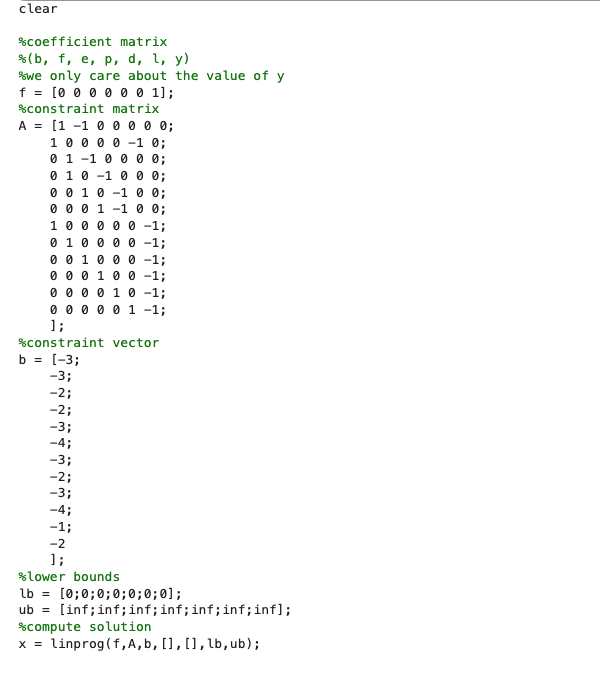
\includegraphics[width=\textwidth]{matlab}
\end{figure}
Here are the results:
\begin{figure}[H]
\centering
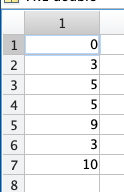
\includegraphics[width=0.2\textwidth]{matlab2}
\end{figure}
This tells us that the optimal point is
\[
(b,f,e,p,d,l,y) =  (0,3,5,5,9,3,10)
\] In particular, this tells us that the optimal value is $y = 10$ weeks.
\newpage
\section*{Problem 2}
First, we must define the variables. Since this is an integer program, we introduce decision variables. Let $p$ be $1$ if we schedule Pedro and $0$ if we do not schedule Pedro. Let $r$ be $1$ if we schedule Roman and $0$ if we do not schedule Roman. Let $b$ be $1$ if we schedule Brittany and $0$ if we do not schedule Brittany. Let $m$ be $1$ if we do schedule Misha and $0$ if we do not schedule Misha. Let $y$ be $1$ if we schedule Yian and $0$ if we do not schedule Yian. Let $a$ be $1$ if we schedule Anasophia and $0$ if we do not schedule Anasophia. Finally, we let $t$ be $1$ if we schedule Ty and $0$ if we do not schedule Ty. Next, we must minimize the total salary. That is, we must minimize the following expression:
\[
30p + 18r + 21b + 38m + 20y + 22a + 9t
\] Now, we must find the constraints. First, we already know that
\[
p,r,b,m,y,a,t \in \{0,1\}
\] since we are assuming that this is an integer program. Furthermore, the problem tells us that at least one lifeguard must be working at all times. First, from $1-2$ PM, Pedro and Roman are available, so we have
\[
p+r \geq 1
\] From $2-3$ PM, Pedro and Roman are available, so we get the same constraint. From $3-4$ PM, Pedro is available, so we have
\[
p \geq 1
\] From $4-5$ PM, Pedro, Brittany, and Misha are available, so we have
\[
p+b+m \geq 1
\] From $5-6$ PM, Brittany, Misha, and Anasophia are available, so we have
\[
b+m+a \geq 1
\] From $6-7$ PM, Brittany, Misha, Yian, and Anasophia are available, so we have
\[
b+m+y+a \geq 1
\] From $7-8$ PM, Misha, Yian, and Anasophia are available, so we have
\[
m+y+a\geq 1
\] From $8-9$ PM, Misha, Yian, and Ty are available, so we have
\[
m+y+t\geq 1
\] 
\newpage
\section*{Problem 3}
The dual linear program is as follows
\begin{align*}
\text{minimize}\quad &4y_1 -2y_2 \\
\text{subject to}\quad &y_1 + y_2 \geq 3\\
&2y_1-y_2 \geq 1\\
&2y_1 + y_2 \geq 4\\
&y_1 - y_2 \geq 1\\
&y_1,y_2 \geq 0
\end{align*}
\subsection*{Part A}
First, we must check that $x^* = [0,1,0,2]^T$ is actually feasible. We have
\[
x_1+ 2x_2 + 2x_3 + x_4 = 0 + 2(1) + 2(0) + 2 = 4 \leq 4
\] and 
\[
x_1 - x_2 + x_3 - x_4 = 0 - 1 + 0 - 2 = -3 \leq -2
\] It is easy to see that the nonnegativity conditions are satisfied.
By the complementary slackness conditions, we have
\begin{align*}
2y_1 - y_2 &= 1\\
y_1 - y_2 &= 1
\end{align*} Since we know that 
\[
x_1 - x_2 + x_3 - x_4 = 0 - 1 + 0 - 2 = -3 < -2
\] we have $y_2 = 0$ so that the two equations become
\begin{align*}
2y_1  &= 1\\
y_1  &= 1
\end{align*} which is impossible. Thus $x^*$ is not optimal.
\subsection*{Part B}
First, we check to see if $x^* = [1,0,0,3]^T$ is actually feasible. We have
\[
x_1 + 2x_2 + 2x_3 + x_4 = 1 + 2(0) + 2(0) + 3 = 4 \leq 4
\] and
\[
x_1-x_2+x_3-x_4 = 1-0+0-3 = -2 \leq -2
\] Thus, the point $x^*$ is feasible. Using the complementary slackness conditions, we find that 
\begin{align*}
y_1 + y_2 &= 3\\
y_1 - y_2 &= 1
\end{align*}
 Adding the two equations gives $y_1 = 2$ so that $y_2 = 1$. Thus, we obtain the point $(y_1,y_2) = (2,1)$. We must check that this point satisfies the other conditions. Notice that
 \[
 2y_1 - y_2  = 2(2) - 1 = 3 \geq 1
 \] and
 \[
 2y_1 + y_2 = 2(2) + 1 = 5 \geq 4
 \] Also, we see that $y_1,y_2 \geq 0$ so this point is feasible for the dual. Thus the point $x^* = [1,0,0,3]^T$ is optimal. We check this as follows:
 \[
 c^T x^* = 3x_1 + x_2 + 4x_3 + x_4 = 3(1) + 0 + 4(0) + 3 = 6
 \] and
 \[
 b^T y^* = 4y_1 - 2y_2 = 4(2) - 2(1) = 6
 \]
\newpage
\section*{Problem 4}
The dual linear program is:
\begin{align*}
\text{minimize}\quad &3y_1 + 2y_2 + 7y_3 + 4y_4\\
\text{subject to}\quad & y_1 + 2y_3 \geq 1\\
& y_2 + 2y_4 \geq 5\\
& y_1 + y_2 - y_3 \geq 3\\
& 3y_1 + y_2 - y_3 + y_4 \geq 6\\
&  3y_3 + 2y_4 \geq 6\\
& y_1,y_2,y_3,y_4 \geq 0
\end{align*} Let us review the complementary slackness conditions. These conditions say that for all $j = 1,\ldots,n$, we have
\[
x^*_j > 0 \implies \sum_{i=1}^m a_{ij}y_i^* = c_j
\] and for all $i = 1,\ldots,m$, we have
\[
\sum_{j=1}^n a_{ij}x_j^* < b_i \implies y_i^* = 0
\] We can rewrite these conditions so that for all $j = 1,\ldots,n$, we have
\[
\sum_{i=1}^m a_{ij}y_i^* > c_j \implies x_j^* = 0
\] and for all $i = 1,\ldots,m$, we have
\[
y_i^* > 0 \implies \sum_{j=1}^n a_{ij} x_j^* = b_i
\] Now, let us see this in practice. First, we substitute $y^* = [1,2,0,3]^T$ into the inequalities in the dual linear program.
\[
y_1 + 2y_3 = 1 + 2(0) = 1
\] and
\[
y_2 + 2y_4 = 2 + 2(3) = 8 > 5
\] and
\[
y_1 + y_2 - y_3 = 1 + 2 - 0 = 3
\] and
\[
3y_1 + y_2 - y_3 + y_4 = 3(1) + 2 - 0 + 3 = 8 > 6
\] and
\[
3y_3 + 2y_4 = 3(0) + 2(3) = 6
\] Now the second and fourth inequalities are both strict so that $x_2 = x_4 = 0$. Next, we know that $y_1,y_2,y_4 > 0$ so that 
\begin{align*}
x_1 + x_3 + 3x_4 &= 3\\
x_2+x_3+x_4 &= 2\\
2x_2 + x_4 + 2x_5 &= 4
\end{align*} Substituting $x_2 = x_4 = 0$ into these equations yields
\begin{align*}
x_1 + x_3&= 3\\
x_3 &= 2\\
2x_5 &= 4
\end{align*}
so that $x_1  = 1$, $x_3 = 2$, and $x_5 = 2$. Thus, we find that the optimal solution $x^* = (1,0,2,0,2)$. We can check this solution as follows. Notice that
\[
c^Tx^* = x_1 + 5x_2 + 3x_3 + 6x_4 + 6x_5 = 1 + 5(0) + 3(2) + 6(0) + 6(2) = 1 + 6 + 12 = 19
\] and
\[
b^Ty^* = 3y_1 + 2y_2 + 7y_3 + 4y_4 = 3(1) + 2(2) + 7(0) + 4(3) = 3 + 4 + 12 = 19
\]
\end{document} 
%\begin{figure}[H]
%\centering
%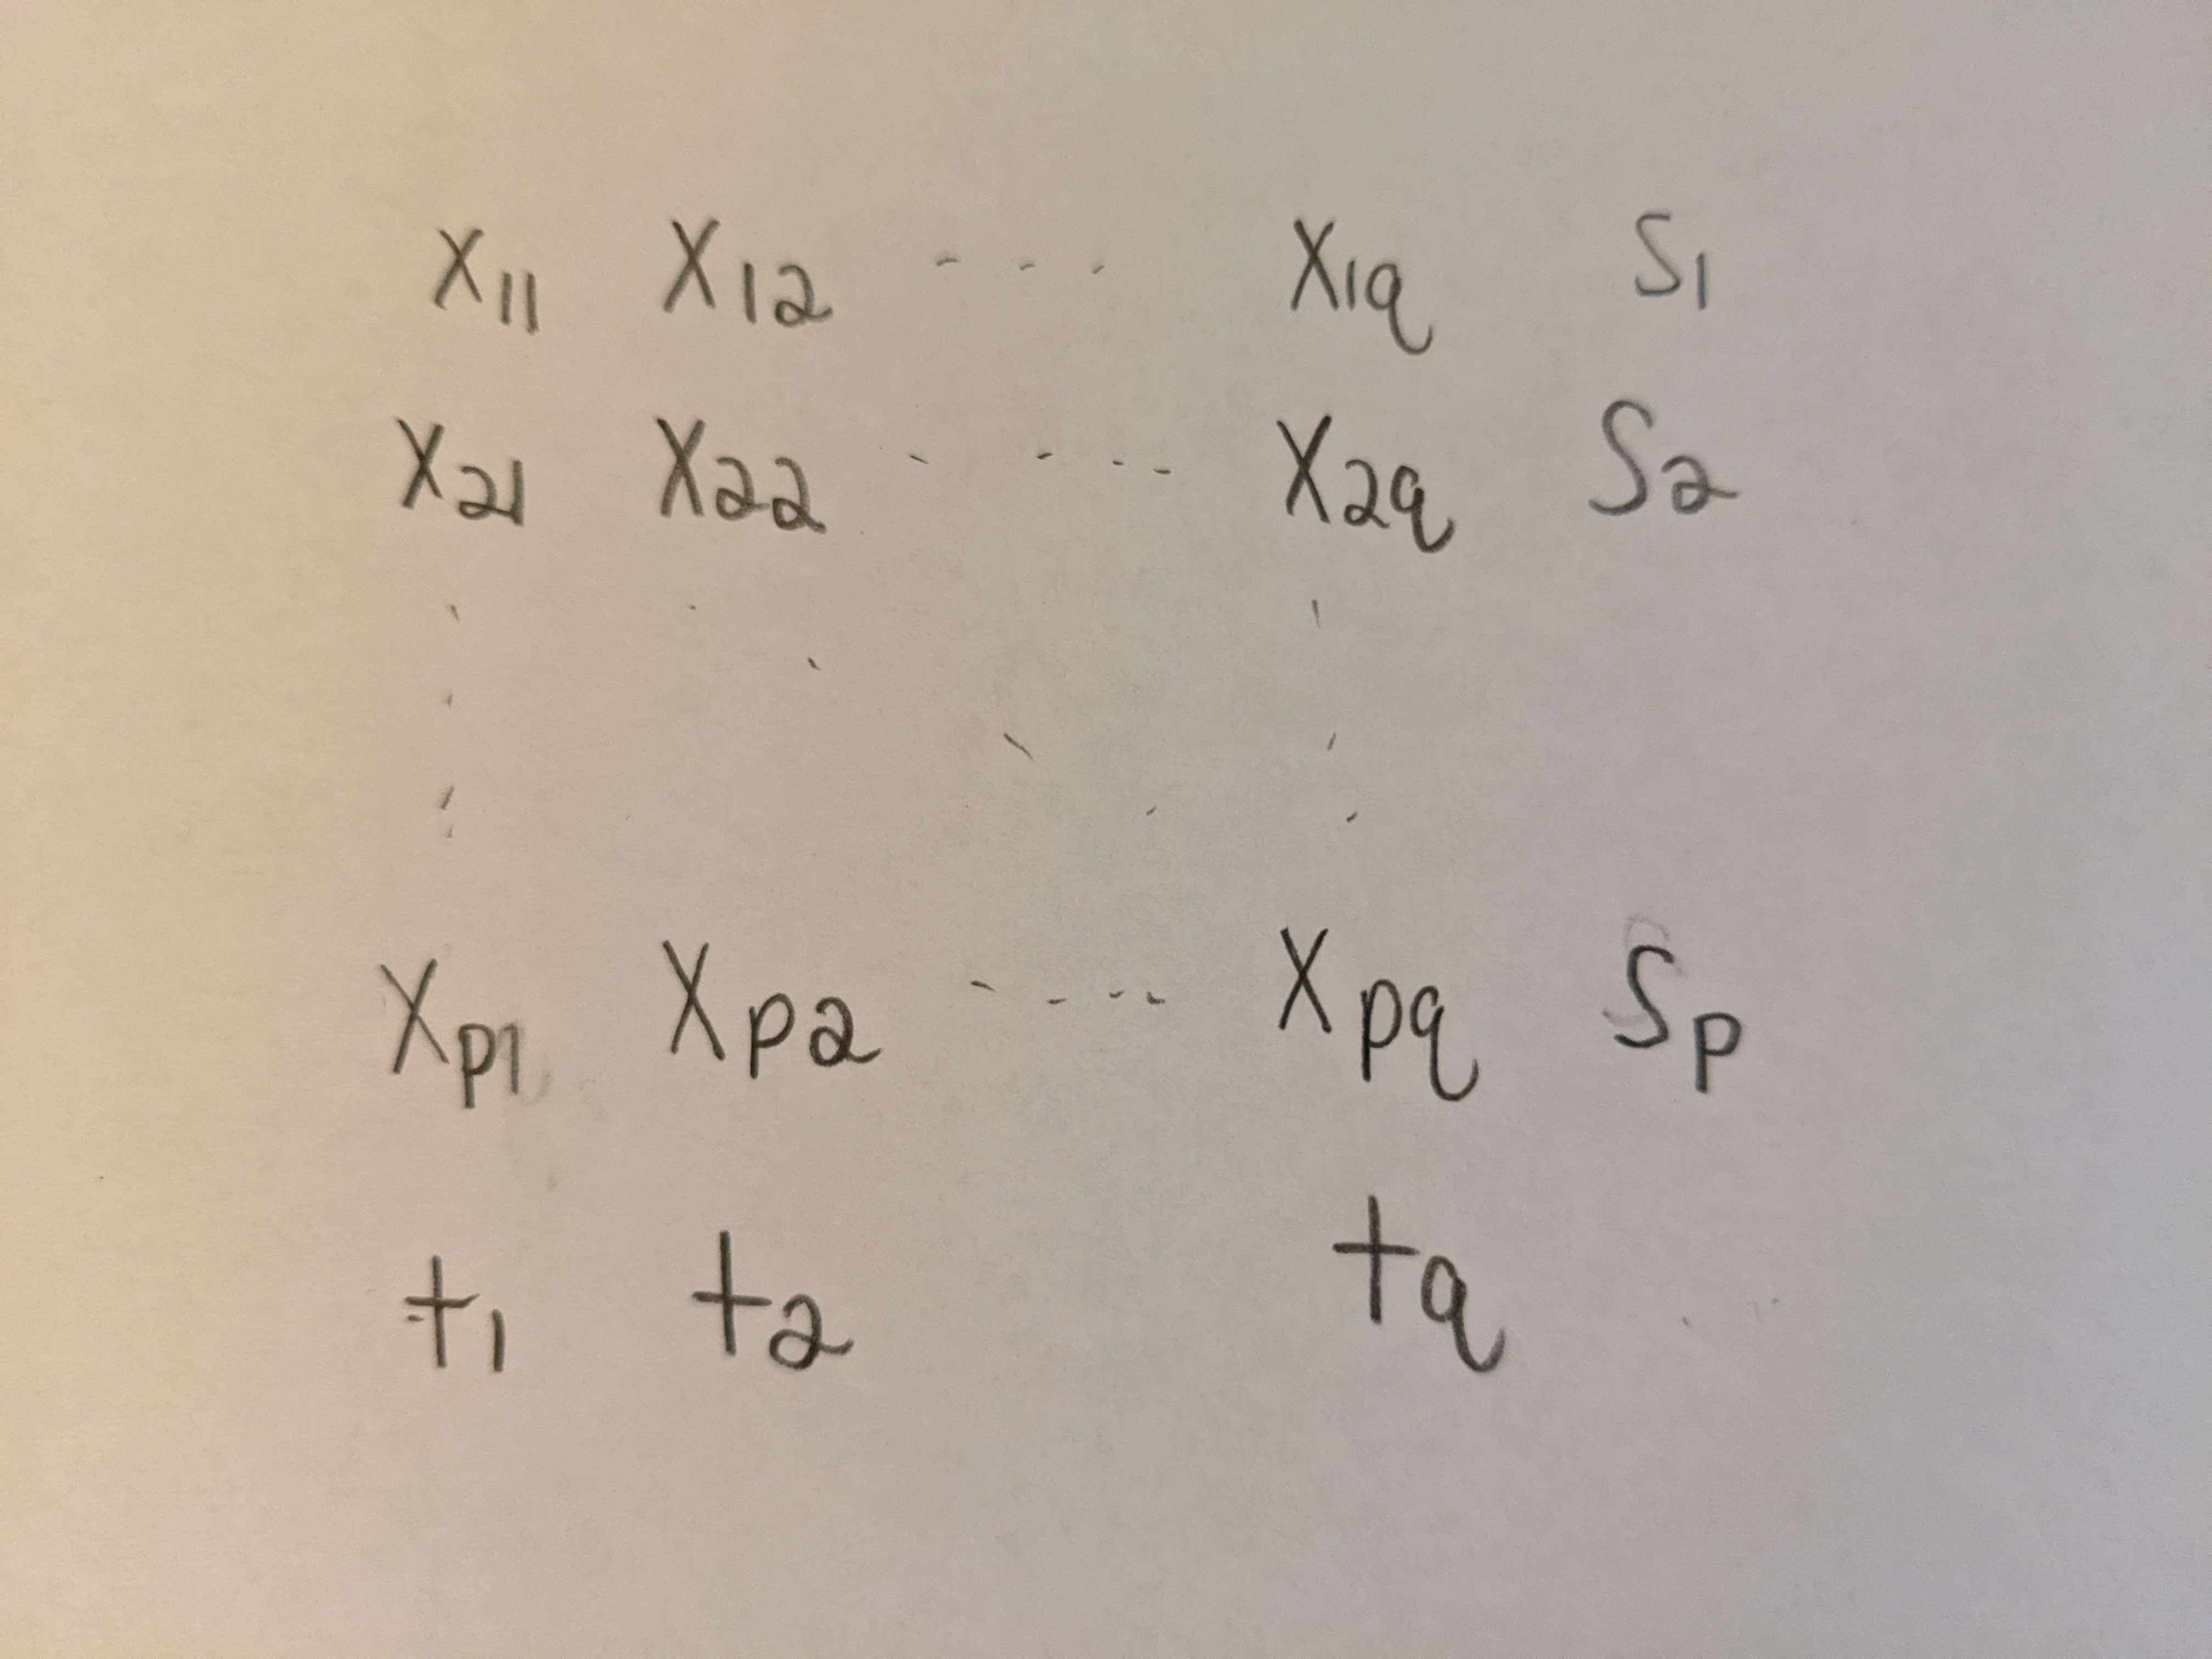
\includegraphics[width=\textwidth]{pic1}
%\end{figure}